\FloatBarrier
\chapter{طراحی آزمایشات}

\section{آماده سازی}
شبیه سازی های آورده شده در این قسمت با استفاده از زبان برنامه پایتون
\LTRfootnote{python}
پیاده سازی شده است. از این رو چه در بخش های کار با داده و آماده سازی دادگان و چه در بخش های پردازش نیاز به دانلود و نصب برخی پکیج های مورد نیاز است. این موارد را به راحتی به کمک ابزار \texttt{pip}
می‌توان نصب کرد. برای این کار ابتدا یک فایل به نام \texttt{requirements.txt}
ایجاد کرده و داخل آن موارد نصبی را می‌نویسیم.


\begin{latin}
\begin{wgetlisting}{requirements.txt}
folium==0.2.1
numpy
tensorflow>=2.3.0
ismrmrd
sigpy
mpi4py
mridata
wget
git+git://github.com/ismrmrd/ismrmrd-python-tools.git
\end{wgetlisting}
\end{latin}

برای نصب نیز کافیست که دستور زیر را در مسیر فایل \texttt{requirements.txt} اجرا کرد.

\begin{latin}%$\bashnumbering$
\begin{lstlisting}[language=bash, frame=none, mathescape=true]
pip install -r requirements.txt 
\end{lstlisting}
\end{latin}









\section{دادگان آزمایش}
در بخش \ref{ch:background|sec:format-storage}
فرمت های گوناگون دادگان توضیح داده شد. در این آزمایش بخش مهمی از دادگان توسط سایت \urlWithoutHttp{mridata.org}
تهیه شده است. در این سایت دیتاست های خام زیادی وجود دارد که با فرمت \lr{ismrmrd}
ذخیره شده اند. همان گونه که در بخش \ref{ch:background|sec:format-storage} اشاره شد، این نوع فرمت برای ذخیره دادگان خام جهت بازسازی مناسب هستند. 




\begin{figure}[t!]
	\centering
	\copyrightbox[b]{
		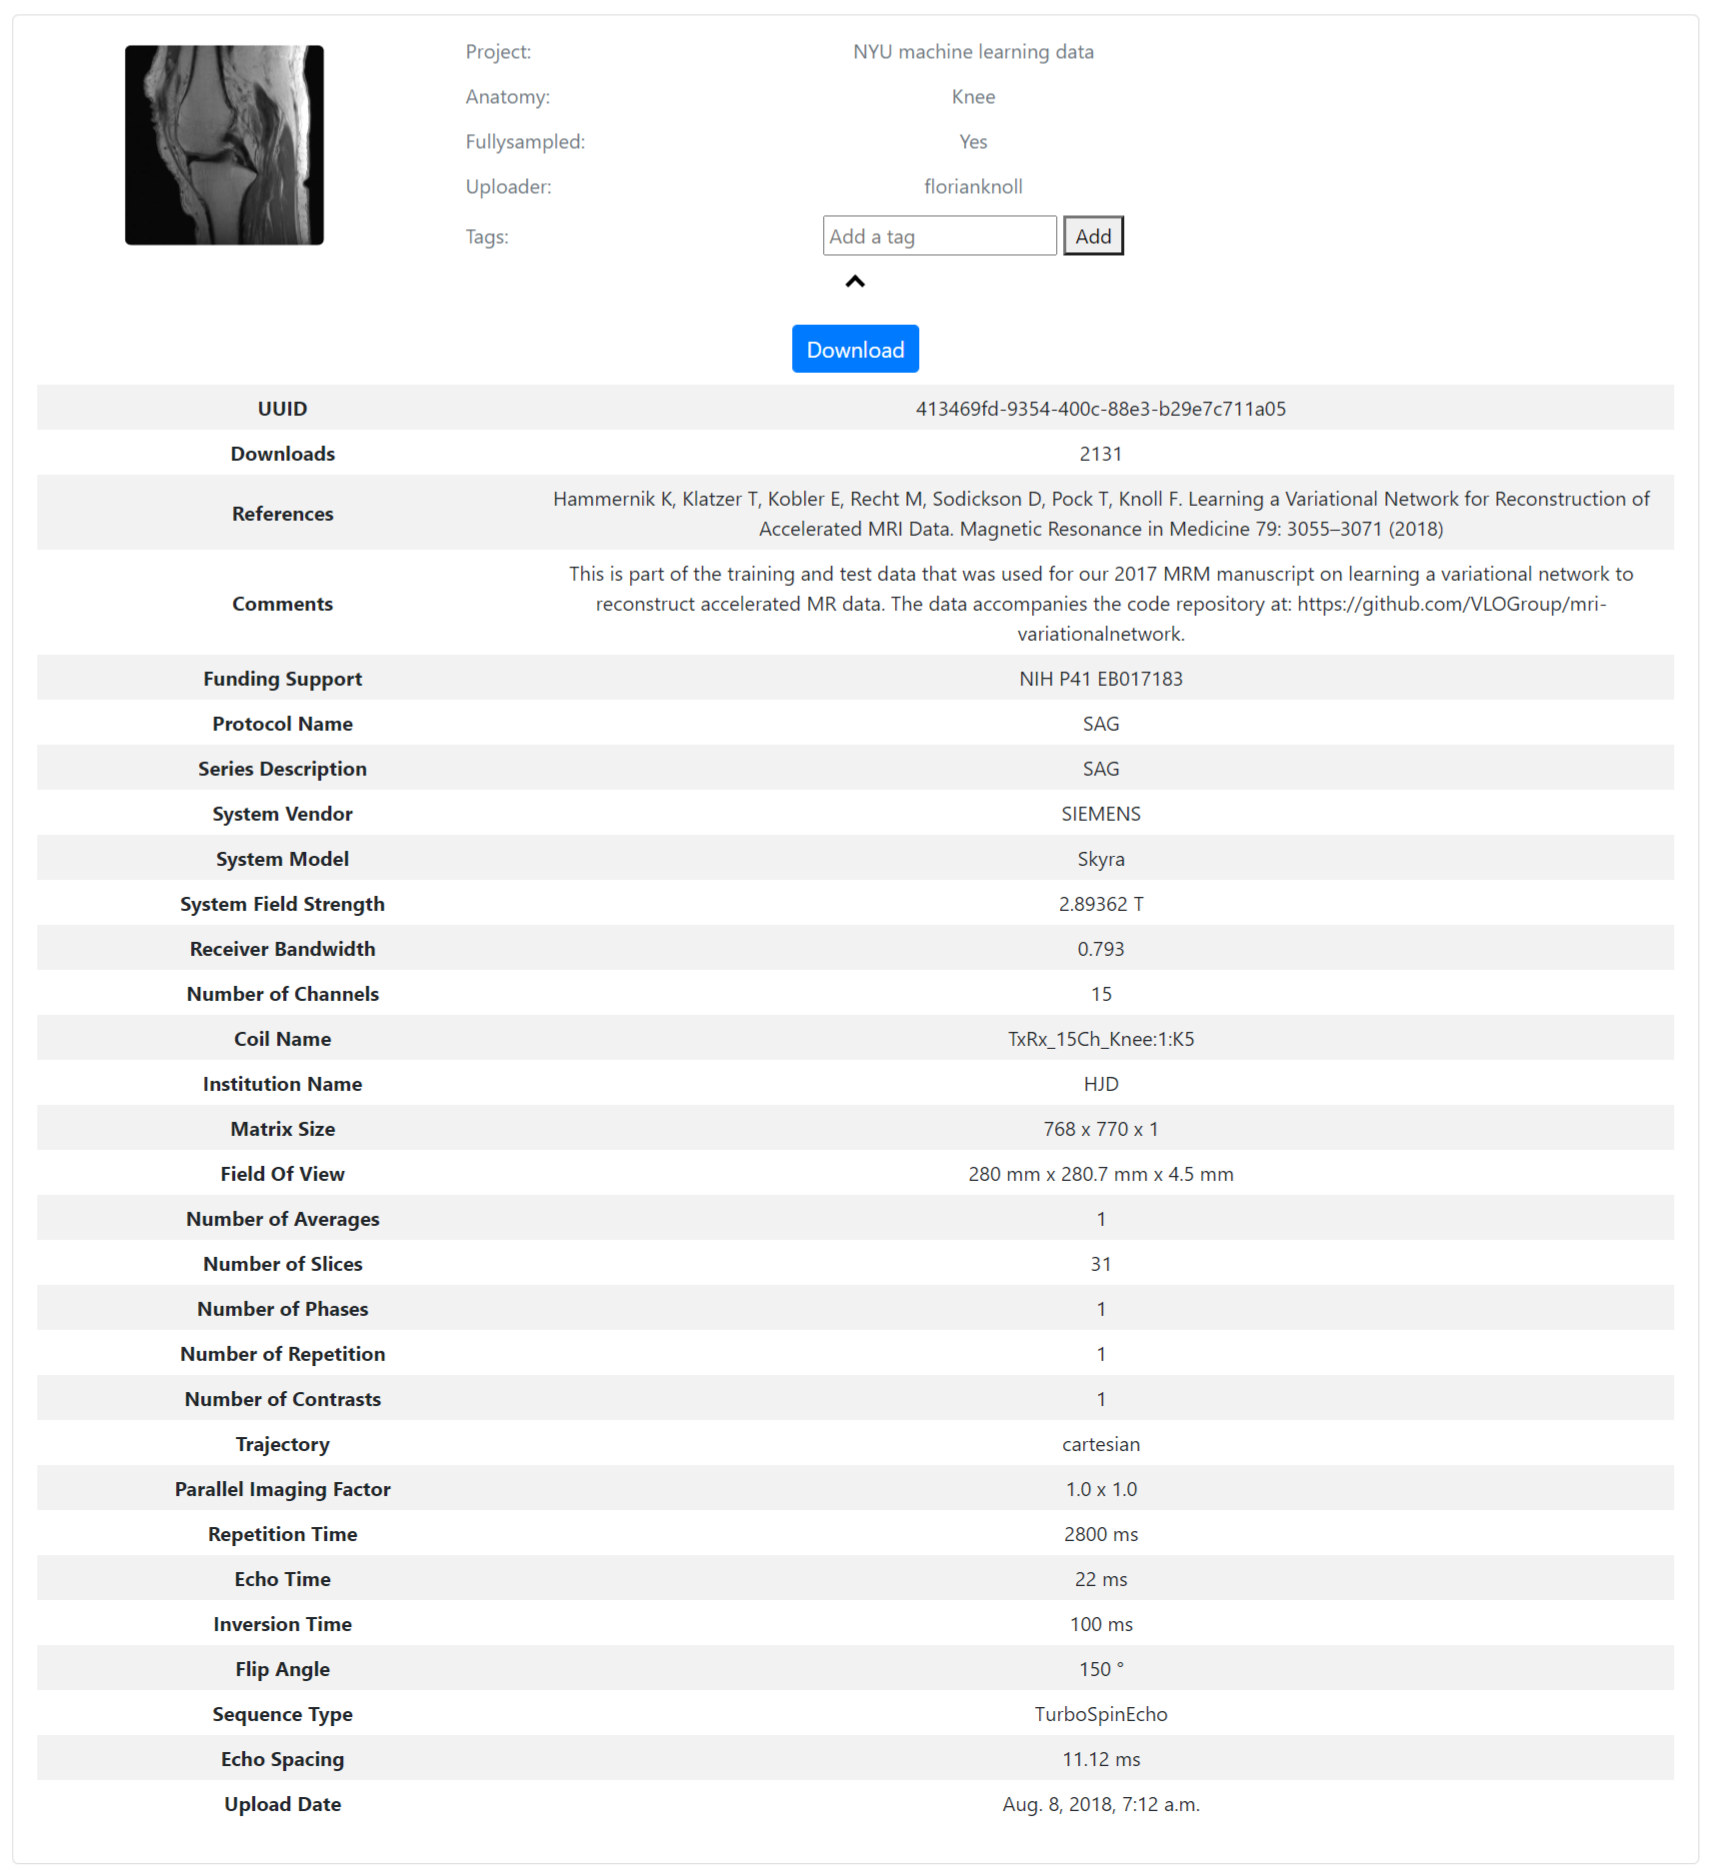
\includegraphics[width=0.9\linewidth]{chapters/chapter-4/figs/mridata-org-fields}
	}{\urlSource{http://mridata.org/list?project=NYU\%20machine\%20learning\%20data}}	
	\removevspace[1]
	\caption{}
	\label{fig:mridata-org-fields}
\end{figure}

شکل \ref{fig:mridata-org-fields}
اطلاعات مورد نیاز جهت دانلود دیتاست مورد نظر را در اختیار ما قرار می‌دهد. ردیف داده‌ی شکل \ref{fig:mridata-org-fields}، 
\lr{UUID}
آن می‌باشد که از آن جهت دانلود این دیتاست استفاده خواهیم کرد. همچنین در آن \lr{trajectory} و \lr{Parallel Imaging Factor}
به ترتیب نوع تراژکتوری اخذ داده(در اینجا کارتزین) و میزان نمونه برداری زیر نرخ (در اینجا نمونه برداری کامل انجام شده است چرا که این پارامتر یک می‌باشد.) را نشان می‌دهد.

برای استخراج جداولی مانند شکل \ref{fig:mridata-org-fields} به شکل یک لیستی از دیتافریم های کتابخانه \texttt{pandas} از کد زیر استفاده شده است:

\begin{latin}
\begin{lstlisting}
import pandas as pd
def mridataorg_to_pandas(url= 'http://mridata.org/list?project=NYU%20machine%20learning%20data'):
	tables = pd.read_html(url)
	tables = pd.concat([t.set_index(0).T for t in tables if (len(t.columns)==2 and any(t.iloc[:,0].str.contains('UUID')))])
	return tables
\end{lstlisting}
\end{latin}



\subsubsection{نحوه دانلود و خواندن داده‌ها}

برای دانلود و استفاده از دادگان این سایت در پایتون بهترین کار این است که از کد زیر استفاده کرد.


\begin{latin}
\begin{lstlisting}
import mridata, pathlib
uuid = 'cc52722b-8649-45b0-a1ea-8727c1687ad5'
dir_output = 'data'
pathlib.Path(dir_output).mkdir(parents=True, exist_ok=True)
mridata.download(uuid, folder=dir_output)
\end{lstlisting}
\end{latin}

پکیج \texttt{mridata}
برای دانلود دیتاست ها از سایت \urlWithoutHttp{mridata.org}
استفاده می‌شود و به \texttt{uuid}
دیتاست جهت انجام این کار نیاز دارد.
سپس برای خواندن این فرمت باید به شیوه زیر عمل کرد:

\begin{latin}
\begin{lstlisting}
import ismrmrd, ismrmrdtools
filename = os.path.join(dir_mridata_org, uuid+".h5")
dset = ismrmrd.Dataset(filename, 'dataset', create_if_needed=False)
header = ismrmrd.xsd.CreateFromDocument(dset.read_xml_header())
enc = header.encoding[0]
\end{lstlisting}
\end{latin}

در کد بالا پکیج \texttt{ismrmrd}
برای خواندن دادگان لازم است و پکیج \texttt{ismrmrdtools}
برای بازسازی تصاویر خام به ما کمک می‌کند. سپس سایز های ماتریس ها را می‌خوانیم.


\begin{latin}
\begin{lstlisting}
# Matrix size
eNx = enc.encodedSpace.matrixSize.x # 768
eNy = enc.encodedSpace.matrixSize.y # = 770
eNz = enc.encodedSpace.matrixSize.z # = 1
rNx = enc.reconSpace.matrixSize.x   # = 384
rNy = enc.reconSpace.matrixSize.y   # = 384
rNz = enc.reconSpace.matrixSize.z   # = 1
\end{lstlisting}
\end{latin}

با مقایسه‌ی این اندازه ماتریس فضای کد شده با ماتریس فضای باز سازی می‌توان دید که در جهت $x$ و جهت $y$ با دو برابر نرخ، نمونه برداری شده است که به اطلاح اورسمپلینگ 
\LTRfootnote{over sampling}
نامیده می‌شود.	سپس اندازه میدان دید را در این دو فضا برحسب میلی متر بدست می‌آوریم. در این صورت می‌توانیم ابعاد واقعی تصویر را مشخص کنیم.

\begin{latin}
\begin{lstlisting}
# Field of View 
eFOVx = enc.encodedSpace.fieldOfView_mm.x # = 280.0
eFOVy = enc.encodedSpace.fieldOfView_mm.y # = 280.700012
eFOVz = enc.encodedSpace.fieldOfView_mm.z # = 4.5
rFOVx = enc.reconSpace.fieldOfView_mm.x   # = 140.0 
rFOVy = enc.reconSpace.fieldOfView_mm.y   # = 140.0
rFOVz = enc.reconSpace.fieldOfView_mm.z   # = 3.0
\end{lstlisting}
\end{latin}
و برای بدست آوردن سایر اطلاعات مفید مانند تعداد اسلایس ها، تکرار ها و کنتراست از کد زیر استفاده می‌کنیم.

\begin{latin}
\begin{lstlisting}
# Number of Slices, Reps, Contrasts, etc.
ncoils = header.acquisitionSystemInformation.receiverChannels # = 15
if enc.encodingLimits.slice != None:
	nslices = enc.encodingLimits.slice.maximum + 1 # = 36
else:
	nslices = 1
if enc.encodingLimits.repetition != None:
	nreps = enc.encodingLimits.repetition.maximum + 1 # = 1
else:
	nreps = 1
if enc.encodingLimits.contrast != None:
	ncontrasts = enc.encodingLimits.contrast.maximum + 1 # = 1
else:
	ncontrasts = 1
\end{lstlisting}
\end{latin}

\subsubsection{نحوه بازسازی تصویر از داده خام}
داده های ارایه شده توسط سایت \urlWithoutHttp{mridata.org}
به صورت خام در فضای \kspace و به فرمت فایل \lr{ismrmrd}
ذخیره شده است.از آنجایی که داده ها نمونه برداری کامل شده اند، نحوه بازسازی به اطلاعات بخش \ref{ch:background}
باز می‌گردد اما از آنجا که کار با این فرمت نیز به همان اندازه پیچیده است، در این قسمت مروری بر نحوه بازساری با استفاده از پایتون خواهد شد. 

\begin{latin}
\begin{lstlisting}
import os
import ismrmrd, ismrmrd.xsd
import numpy as np
from ismrmrdtools import show, transform

remove_oversampling_x = True
# Initialiaze a storage array
all_data = np.zeros((nreps, ncontrasts, nslices, ncoils, eNz, eNy, rNx if remove_oversampling_x else eNx),  dtype=np.complex64)

# Loop through the rest of the acquisitions and stuff
for acqnum in range(firstacq,dset.number_of_acquisitions()):
	acq = dset.read_acquisition(acqnum)
	# TODO: this is where we would apply noise pre-whitening
	# Remove oversampling if needed
	if eNx != rNx:
		xline = transform.transform_kspace_to_image(acq.data, [1])
		x0 = (eNx - rNx) // 2
		x1 = (eNx - rNx) // 2 + rNx
		xline = xline[:,x0:x1]
		acq.resize(rNx,acq.active_channels,acq.trajectory_dimensions)
		acq.center_sample = rNx//2
		# need to use the [:] notation here to fill the data
		acq.data[:] = transform.transform_image_to_kspace(xline, [1])
	# Stuff into the buffer
	rep = acq.idx.repetition
	contrast = acq.idx.contrast
	slice = acq.idx.slice
	y = acq.idx.kspace_encode_step_1
	z = acq.idx.kspace_encode_step_2
	all_data[rep, contrast, slice, :, z, y, :] = acq.data
\end{lstlisting}
\end{latin}




\begin{latin}
\begin{lstlisting}
import os
import ismrmrd
import ismrmrd.xsd
import numpy as np
import matplotlib.pyplot as plt
from ismrmrdtools import show, transform

# Initialiaze a storage array
# Reconstruct images
images = np.zeros((nreps, ncontrasts, nslices, eNz, eNy, rNx if remove_oversampling_x else eNx),  dtype=np.float32)
fig = plt.figure()
plt.xlim([0,1]); plt.ylim([0,1]);

# Loop through the rest of the acquisitions and stuff
for acqnum in range(firstacq,dset.number_of_acquisitions()):
acq = dset.read_acquisition(acqnum)

# Stuff into the buffer
rep = acq.idx.repetition
contrast = acq.idx.contrast
slice = acq.idx.slice
y = acq.idx.kspace_encode_step_1
z = acq.idx.kspace_encode_step_2
# print(y,z)
all_data[rep, contrast, slice, :, z, y, :] = acq.data
# display.clear_output(wait=True)
# x = np.arange(100)
# y = np.sin(x + np.random.rand())
# plt.plot(x, y, '-r')
# plt.show()
\end{lstlisting}
\end{latin}




\begin{latin}
\begin{lstlisting}
# Reconstruct images
images = np.zeros((nreps, ncontrasts, nslices, eNz, eNy, rNx), dtype=np.float32)
for rep in range(nreps):
	for contrast in range(ncontrasts):
		for slice in range(nslices):
			# FFT
			if eNz>1: #3D
				im = transform.transform_kspace_to_image(all_data[rep, contrast,slice,:,:,:,:], [1,2,3])
			else: #2D
				im = transform.transform_kspace_to_image(all_data[rep, contrast,slice,:,0,:,:], [1,2])
			# Sum of squares
			im = np.sqrt(np.sum(np.abs(im) ** 2, 0))
				
			# Stuff into the output
			if eNz>1: #3D
				images[rep,contrast,slice,:,:,:] = im
			else: #2D
				images[rep,contrast,slice,0,:,:] = im
# Show an image
show.imshow(np.squeeze(images[0,0,0,:,:,:]))
\end{lstlisting}
\end{latin}


\begin{figure}[t!]
	\centering
	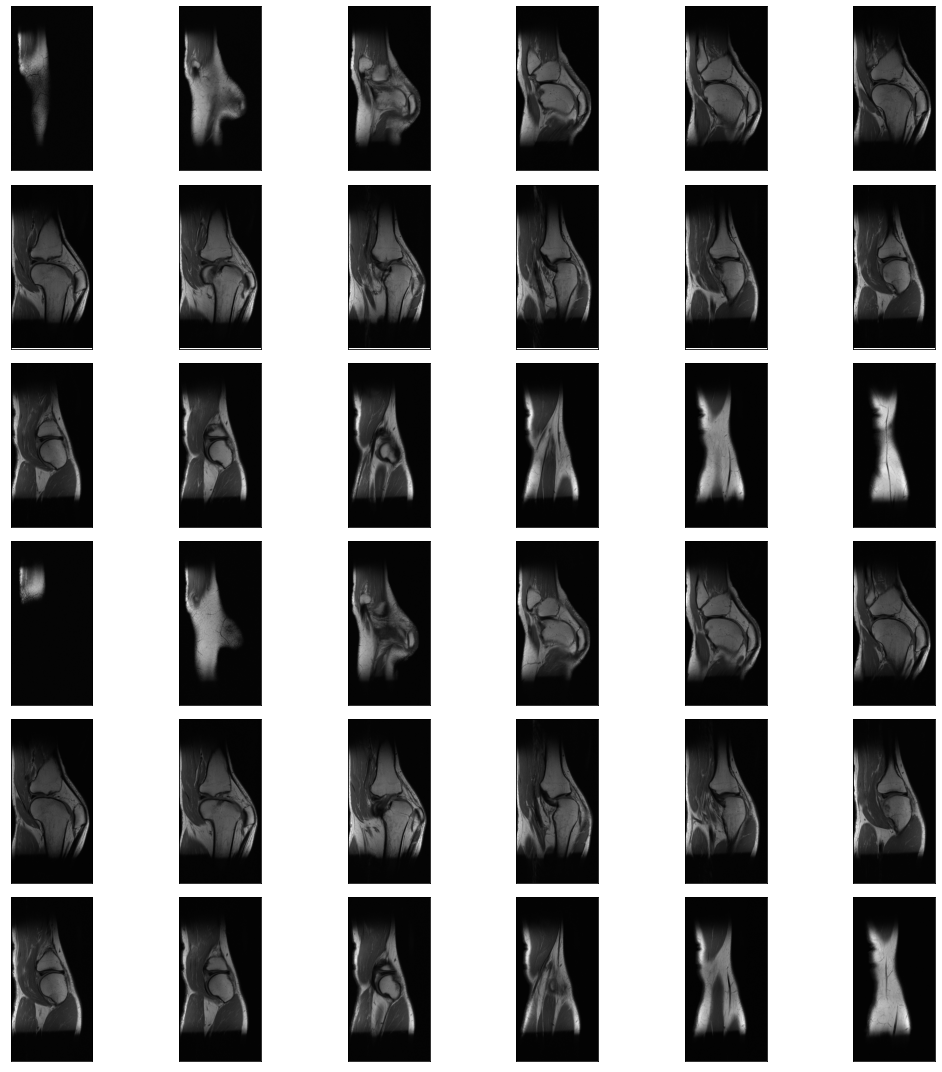
\includegraphics[width=0.6\linewidth]{chapters/chapter-4/figs/result-36-plots-data-load}
	\caption{تصاویر بازسازی شده از داده خام و نمونه برداری شده کامل}
	\label{fig:result-36-plots-data-load}
\end{figure}

خروجی حاصل این کد در شکل \ref{fig:result-36-plots-data-load}
نمایش داده شده است.
همچنین تصویر \ref{fig:413469fd-9354-400c-88e3-b29e7c711a05}
تفاوت حالتی که نمونه برداری بیش از حد حذف شده است با حالتی که حذف نشده است را به نمایش گذاشته است. توجه شود که هنگامی که نمونه برداری بیش از حد حذف نشده باشد، یک لایه گذاری صفر
\LTRfootnote{zero-padding}
در راستای $x$ اتفاق می‌افتد. در حقیقت با حذف این موضوع، اطلاعاتی که حذف می‌شود مربوط به بخش های سیاه اطراف شئ هستند و اطلاعات خود شئ محفوظ باقی می‌ماند.

\begin{figure}[t!]
	\centering
	\subfigure[تصاویر بازسازی شده همراه با نمونه برداری بیش از حد]{
		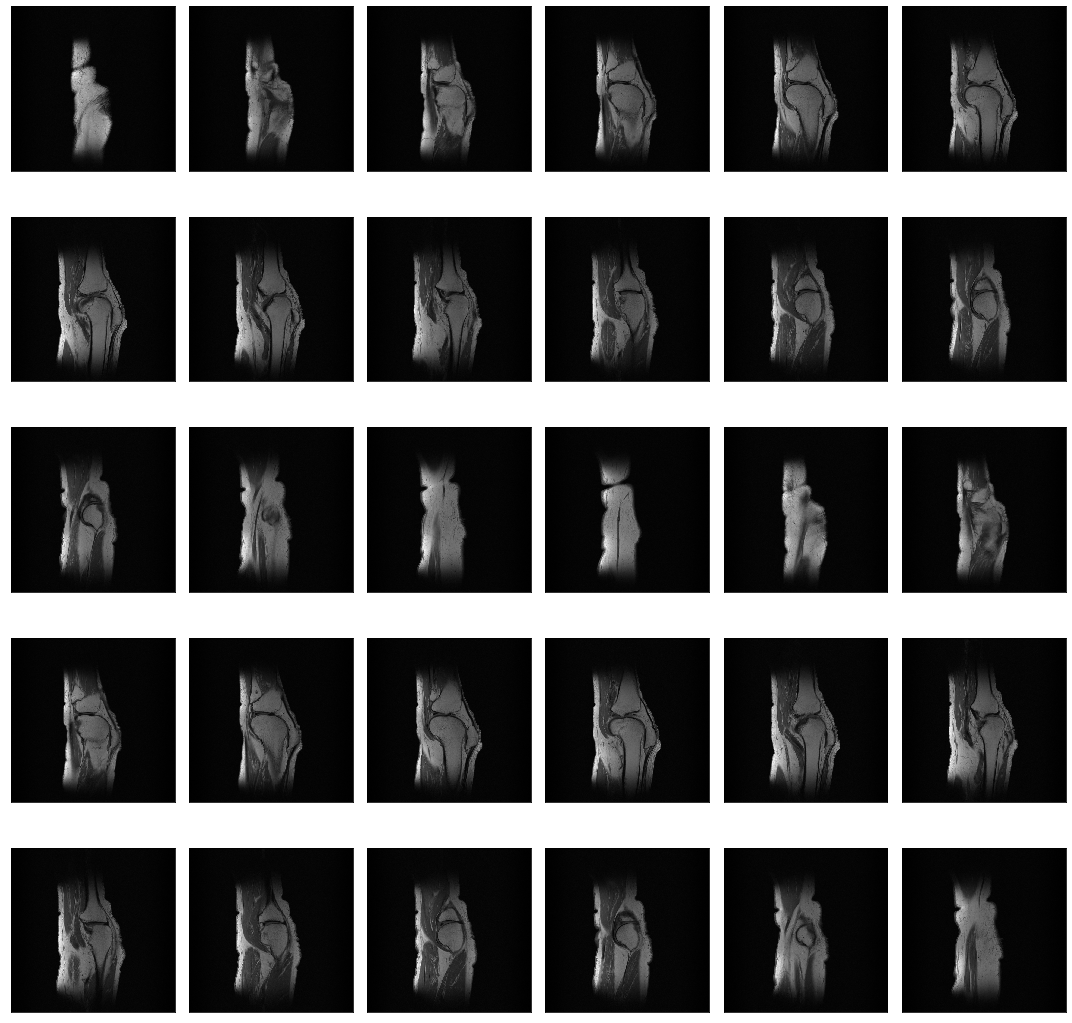
\includegraphics[height=0.43\linewidth]{chapters/chapter-4/figs/413469fd-9354-400c-88e3-b29e7c711a05-withOversampling}
		\label{subfig:413469fd-9354-400c-88e3-b29e7c711a05-with-oversampling}}
	\hfill
	\subfigure[تصاویر بازسازی شده همراه با حذف نمونه برداری بیش از حد]{
		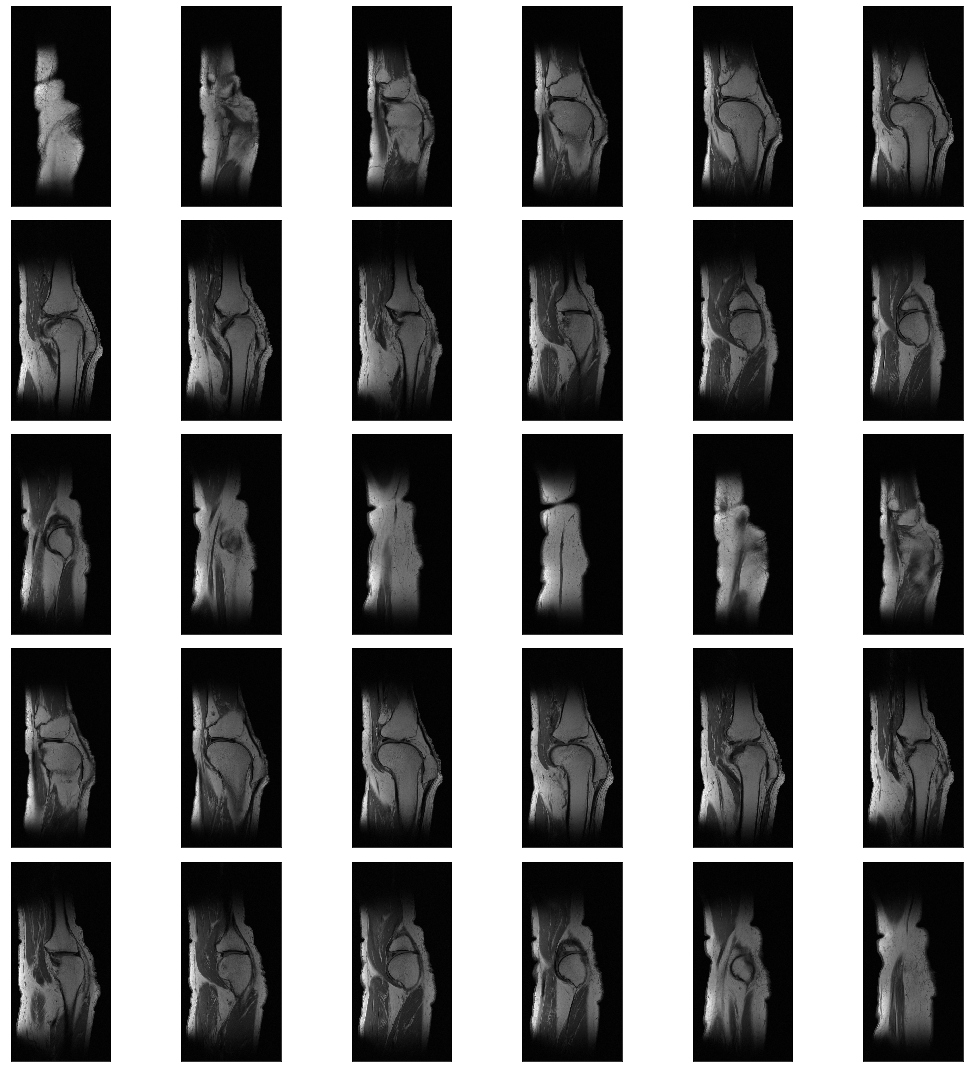
\includegraphics[height=0.43\linewidth]{chapters/chapter-4/figs/413469fd-9354-400c-88e3-b29e7c711a05-withoutOversampling}
		\label{subfig:413469fd-9354-400c-88e3-b29e7c711a05-without-oversampling}}
	\caption{مقایسه تفاوت تصاویر خروجی برای حالت هایی که نمونه برداری بیش از حد حذف شده است و حالاتی که حذف نشده است. }
	\label{fig:413469fd-9354-400c-88e3-b29e7c711a05}
\end{figure}




\subsection{سیستم و فایل های اجرایی}
داده هایی به فرمت \lr{ismrmrd}
برای پردازش به هیچ عنوان مناسب نیستند. اگرچه این داده ها، داده های خام فضای \kspace
هستند اما ساخت یک ماتریس \kspace از روی این دادگان خام امری زمان بر است و برای یک داده به حجم $1.5 Gb$ 
بیشتر از $1.5$ دقیقه زمان می‌برد تا یک ماتریس \kspace پر شود. برای غلبه به این مشکلات داده ها و پیش پردازش و شناخت داده های \kspace یک مجموعه فایل به فرمت \lr{jupyter notebook (ipynb)}
تهیه شده است که برروی گیت‌هاب 
\LTRfootnote{
\url{https://github.com/MohammadRaziei/mri-reconstruction/tree/master/python}
}
قرار داده شده است. فایل 
\href{https://github.com/MohammadRaziei/mri-reconstruction/blob/master/python/requirements.txt}{requirements.txt}
تمامی کتابخانه‌های مورد استفاده را در هردو بخش پردازش و پیش پردازش شامل می‌شود. (البته برای نصب کتابخانه \lr{cupy} به صورت دستی اقدام شود.)

برای اجرای فایل های مرتبط با پیش پردازش از سیستم شخصی دارای \lr{GPU}
مدل \lr{GeForce GTX 1050 Ti}
و با کمک کتابخانه هایی مانند \lr{tensorflow}
 و \lr{cupy}
استفاده شده است.

برای بخش پردازشی نیز از سیستم آزمایشگاه پردازش سیگنال تحت نظارت دکتر آرش امینی استفاده شده است که 
دارای \lr{GPU}
مدل \lr{GeForce GTX 1080 Ti}
 استفاده شده است چرا که 11 گیگابایت حافظه‌ی گلوبال دارد و می‌تواند یک \lr{batch}
از داده را مورد پردازش قرار دهد. همچنین از سرویس های آنلاین \lr{Colab}
و  \lr{Kaggle}
 نیز برای این بخش استفاده شده است و داده های ورودی شبکه عصبی پس از انجام پیش پردازش بروی دیتاست \lr{Kaggle}
 \LTRfootnote{\url{https://www.kaggle.com/mohammadraziei/mridata-dataset/}}
نیز قرار داده شده است.



\subsection{پیش پردازش}
همانطور که گفته شد ساخت ماتریس \kspace داده های \lr{ismrmrd}
کار زمان‌گیری است. همچنین این فایل ها اطلاعات زیادی را شامل می‌شود که برخی از آن ها در بازسازی استفاده ای ندارند. از این رو فایل 
\href{https://github.com/MohammadRaziei/mri-reconstruction/blob/master/python/ismrmrd_to_npz.ipynb}{\texttt{ismrmrd\_to\_npz.ipynb}}
ایجاد شده است که با استفاده از دو کتابخانه اصلی \lr{ismrmrd}
 و \lr{cupy}
با سرعت بالا ماتریس \kspace را از روی داده های خام \lr{ismrmrd}
می سازد. سپس این ماتریس را به ماتریس های کتابخانه \lr{numpy}
تبدیل میکند و به همراه تمام اطلاعات اضافی که در بازسازی کمک می‌کند درون فرمت \texttt{npz}
ذخیره میکند با این کار جحم دیتا به حدود 300 الی 400 مگابایت کاهش پیدا می‌کند و زمان لود آن نیز زیر یک ثانیه خواهد بود بنابراین این کار از هر نظر  مزیت محسوب میشد.


سپس فایل 
\href{https://github.com/MohammadRaziei/mri-reconstruction/blob/master/python/tf_preprocessing.ipynb}{\texttt{tf\_preprocessing.ipynb}}
را اجرا می‌کنیم. از آنجایی که ابعاد ماتریس \kspace در داده های مختلف متقاوت است. این فایل ابتدا اطلاعات اضافی همه‌ی داده‌ها را لود می‌کند و سپس بیشینه مقدار اندازه‌ی تصویر را به همراه یک حاشیه‌ی صفر پیدا می‌کند. مقدار $Nx=400$ و $Ny=640$ از بزرگترین ابعاد داده ها
($\max (Nx, Ny) = (384, 616)$) 
مقداری بزرگتر است. این حاشیه‌ی صفر برای ملاحظات پیاده سازی شبکه های عصبی در نظر گرفته شده است. سپس تمامی داده ها لود شده و اسلایس های آن ها از یکدیگر جدا میشود و هرکدام جداگانه حاشیه‌ی صفر 
\LTRfootnote{zero-padding}
می‌شود.
















